% #######################################
% ########### FILL THESE IN #############
% #######################################
\def\mytitle{Coursework Report}
\def\myauthor{Maria Luque Anguita}
\def\contact{40280156@napier.ac.uk}
\def\mymodule{Advanced Web Technologies (SET09103)}
% #######################################
% #### YOU DON'T NEED TO TOUCH BELOW ####
% #######################################
\documentclass[10pt, a4paper]{article}
\usepackage[a4paper,outer=1.5cm,inner=1.5cm,top=1.75cm,bottom=1.5cm]{geometry}
\twocolumn
\usepackage{graphicx}
\graphicspath{{./images/}}
%colour our links, remove weird boxes
\usepackage[colorlinks,linkcolor={black},citecolor={blue!80!black},urlcolor={blue!80!black}]{hyperref}
%Stop indentation on new paragraphs
\usepackage[parfill]{parskip}
%% Arial-like font
\usepackage{lmodern}
\renewcommand*\familydefault{\sfdefault}
%Napier logo top right
\usepackage{watermark}
%Lorem Ipusm dolor please don't leave any in you final report ;)
\usepackage{lipsum}
\usepackage{xcolor}
\usepackage{listings}
%give us the Capital H that we all know and love
\usepackage{float}
%tone down the line spacing after section titles
\usepackage{titlesec}
%Cool maths printing
\usepackage{amsmath}
%PseudoCode
\usepackage{algorithm2e}

\titlespacing{\subsection}{0pt}{\parskip}{-3pt}
\titlespacing{\subsubsection}{0pt}{\parskip}{-\parskip}
\titlespacing{\paragraph}{0pt}{\parskip}{\parskip}
\newcommand{\figuremacro}[5]{
    \begin{figure}[#1]
        \centering
        \includegraphics[width=#5\columnwidth]{#2}
        \caption[#3]{\textbf{#3}#4}
        \label{fig:#2}
    \end{figure}
}

\lstset{
	escapeinside={/*@}{@*/}, language=C++,
	basicstyle=\fontsize{8.5}{12}\selectfont,
	numbers=left,numbersep=2pt,xleftmargin=2pt,frame=tb,
    columns=fullflexible,showstringspaces=false,tabsize=4,
    keepspaces=true,showtabs=false,showspaces=false,
    backgroundcolor=\color{white}, morekeywords={inline,public,
    class,private,protected,struct},captionpos=t,lineskip=-0.4em,
	aboveskip=10pt, extendedchars=true, breaklines=true,
	prebreak = \raisebox{0ex}[0ex][0ex]{\ensuremath{\hookleftarrow}},
	keywordstyle=\color[rgb]{0,0,1},
	commentstyle=\color[rgb]{0.133,0.545,0.133},
	stringstyle=\color[rgb]{0.627,0.126,0.941}
}

\thiswatermark{\centering \put(336.5,-38.0){\includegraphics[scale=0.8]{logo}} }
\title{\mytitle}
\author{\myauthor\hspace{1em}\\\contact\\Edinburgh Napier University\hspace{0.5em}-\hspace{0.5em}\mymodule}
\date{}
\hypersetup{pdfauthor=\myauthor,pdftitle=\mytitle,pdfkeywords=\mykeywords}
\sloppy
% #######################################
% ########### START FROM HERE ###########
% #######################################
\begin{document}
	\maketitle
	\begin{abstract}
	    The aim of this coursework is to demonstrate my understanding of the Python Flask micro-framework by creating a prototype web application for an online directory about a given subject. The subject here is food, hence why the webpage's title is 'Realfooding' and encourages people to start eating healthier. Food can be divided in real food or ultra-processed food. My web page explains the difference between them and contains many recipes and meal plans depending on the user's lifestyle, where everything is linked to make sure that every ingredient is explained and shows its benefits and drawbacks. Users can also leave doubts or comments that the web owner can then read in the Contact area and answer them.
	\end{abstract}


	\section{Introduction}
	My Realfooding web-app starts with a clear and easy to navigate display where the user can choose what is it that they want to read about, or if they want to get in touch with the specialist. As we scroll down more options appear while the image is still to make it easier to read the options.

	\includegraphics[width=8.5cm]{index.jpg}

    \textbf{Figure 2 Navigation diagram}
    \vspace{2mm}

    From there, we can go to different pages:
    \begin{itemize}
        \item Real food: contains different options to read about, like fruit, vegetables, fish and meat and others. Within those pages, the user can go and find even more information about every specific product that appears. This part contains the base information that then can be accessed from other parts of the web-app, i.e. since it contains aliments, all other recipes and food explanations have links to the aliment here.
        \item Ultra processed products: has information about what they are, why they are bad for us and examples.
        \item Meal plan: this page is the most informative one, it contains options to see different healthy and easy recipe ideas for breakfast, lunch, dinner or snacks, as well as a list of all the recipes there are in the web.
        \item Grocery Shopping: If there is no junk food at home, no one will eat junk food. These grocery shopping lists help people get only what they need and not more. It is divided in 3 options: diet, to lose weight; sports, to gain weight with a specific diet accompanied by doing sports; and events, which contains ideas for recipes that you can use for parties, since parties are normally related with chocolate and many ultra-processed foods.
        \item Contact: this last part is used for users to contact the specialist for any doubts or comments. The specialist will then read them and reply to them.
    \end{itemize}


    \section{Design}

    The web is divided just like the hierarchy shows in Appendix 1. All the objects such as aliments, recipes and customer doubts are saved in Json files. The web will allow you to move between base aliments or recipes, which also contain links to the aliments themselves used in that recipe.

    Before starting to code anything I read various articles about how a good webpage is structured, where I found this quote: "DESIGNING WEB SOFTWARE IS DIFFERENT THAN DESIGNING WEBSITES[1]". This amazing website told me what steps to follow to start designing both, my website design and its software.

    Firstly, I started by creating an application flow, the quickest possible route to allow the user to get to where it wants and all the possible routes and endpoints there would be. Finally, I took my idea from rough sketches to a polish interface and a very effective program.

    All the objects are created in Json files, because they are an easy way to add, edit or remove objects without having to set up an entire database. The admin, when logged in, is the only person allowed to add, edit or remove any of them. Users don't even have the option to do so, as the buttons only appear when logged in.

    All the images in the web-app are made by me, using Canva[3], to which I had to subscribe to be able to use the premium features which allowed me to download the images in png format so the images would be circles instead of squares and to be able to see the background.

    Explaining how and why your web-app is structured the way it is. This section should include a navigation map for the URL hierarchy of your web-app.

    \section{Enhancements}

    In the next months I will be improving my web-app and adding new features that will make it more usable. Some of the ideas I thought for improvements came from my research on how to analyse and enhance a website[2].

    To start with, you can search in my website by writing what you want to find in the URL, but users don't normally use it, so adding a search space will be vital and way easier for users to find exactly what they're looking for instead of going page by page until they find it.

    Even though my website is functional with JSON files and they are easy to use, I will improve it by creating a database and saving everything there. JSON was never designed to handle anything like concurrent connections or any sort of data manipulation, since its own function is to represent data, not to manage it. The database will be used for storing data, and the objects will be sent as JSON.

    Another feature that I think is vital for a website is making it responsive, so it has a clear view on a mobile web browser, and it is also recommended by Google, which agrees that responsive web design is the industry's best practice.

    Allowing users to log in might also be helpful if they want to view all their doubts or save specific pages. Security must be improved in order to save their information.

    Describing the features that you would add or improve.

    \section{Critical Evaluation}

    For this part of the report, I base my critical evaluation in a published article on how to evaluate webpages[4] and my personal assessment.

    First of all, the web-app is designed so that if the user writes the wrong url or finds something that doesn't exist, the web won't crash. It has a very entertaining 404 error handler page.

    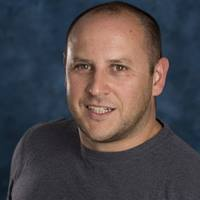
\includegraphics[width=8.5cm]{error.jpg}

    \textbf{Figure 2 Navigation diagram}
    \vspace{2mm}

    \begin{lstlisting}[caption = How error pages are handled]
    @app.errorhandler(404)
    def page_not_found(e):
        return render_template('404error.html'), 404
    \end{lstlisting}

    For the login functionality I used an object called session which allows me to store information specific to a user from one request to another[5]. I included a secret key to make sure that even though the user could look at the contents of my cookie, thay can't modify it unless they know the secret key used for signing. To create the secret key I used python's \textit{urandom(size)} which returns a string of size random bytes suitable for cryptographic use[6].

    \begin{lstlisting}[caption = How secret key is created]
    app = Flask(__name__)
    app.secret_key = os.urandom(12)
    \end{lstlisting}

    Something that makes my web-app efficient is that there are no repeated loops in my code. If something is repeated twice, a function could make it only appear once. For example, the way I retrieve information from the JSON files is through a funcion called \textit{findFood(search)} through which I pass the object to find. This was useful since those objects can be found from anywhere in the web, and if the object was not found, an appropriate error handler initiated. Another function called \textit{generateID(filename)} takes in a JSON file, and generates the next id number making sure none of them were repeated and overlapped. This way I was able to add objects to the files without any crashes.

    This is about what you built and should explain the features of the web-app that you feel work well, or work poorly, and why.
doubts correctly saved to json file
json files make it easy to bring and use information
downloading files

 excellent level of functionality, both in terms of the number of
features and their quality of implementation
 have effectively evaluated

    \section{Personal Evaluation}
    This is about how you perfomed. You should reflect upon what you learned,
the challenges you faced, the methods you used to overcome challenges, and how you feel you performed.

    \section{References}
    If you have used additional resources then these should be cited. Please acknowledge all sources of help and material. If there is anything included that was not written by you for this module, then you should indicate that within this section

    Designing Web Applications

    [1] \url{http://nathanbarry.com/webapps/}

    [2] \url{https://tsquaredmarketing.com/website-enhancement/}

    [3] \url{https://www.canva.com/}

    [4] \url{https://lrweb.beds.ac.uk/applied-soc-studies/Webresources/evaluate-a-webpage}

    [5] \url{http://flask.pocoo.org/docs/1.0/quickstart/}

    [6] \url{https://docs.python.org/3/library/os.html}

https://en.wikipedia.org/wiki/Fruit#Nutritional_value
https://www.healthline.com/nutrition/how-much-fruit-per-day
https://iplaybaby.com/whole-baby-resource/info/types-of-fruits/
https://www.vegetables.co.nz/vegetables-a-z/
https://www.quora.com/Why-do-we-need-to-eat-vegetables
http://www.carballeira.com/en/white-fish-or-blue-fish/
https://www.safefood.eu/Healthy-Eating/What-is-a-balanced-diet/The-Food-Pyramid/Breads,-cereals-and-potatoes.aspx
https://mindovermunch.com/2018/05/03/are-processed-foods-bad/
https://www.sproutright.com/blog/index.php/5-reasons-you-need-snacks/

    \section{Appendices}

    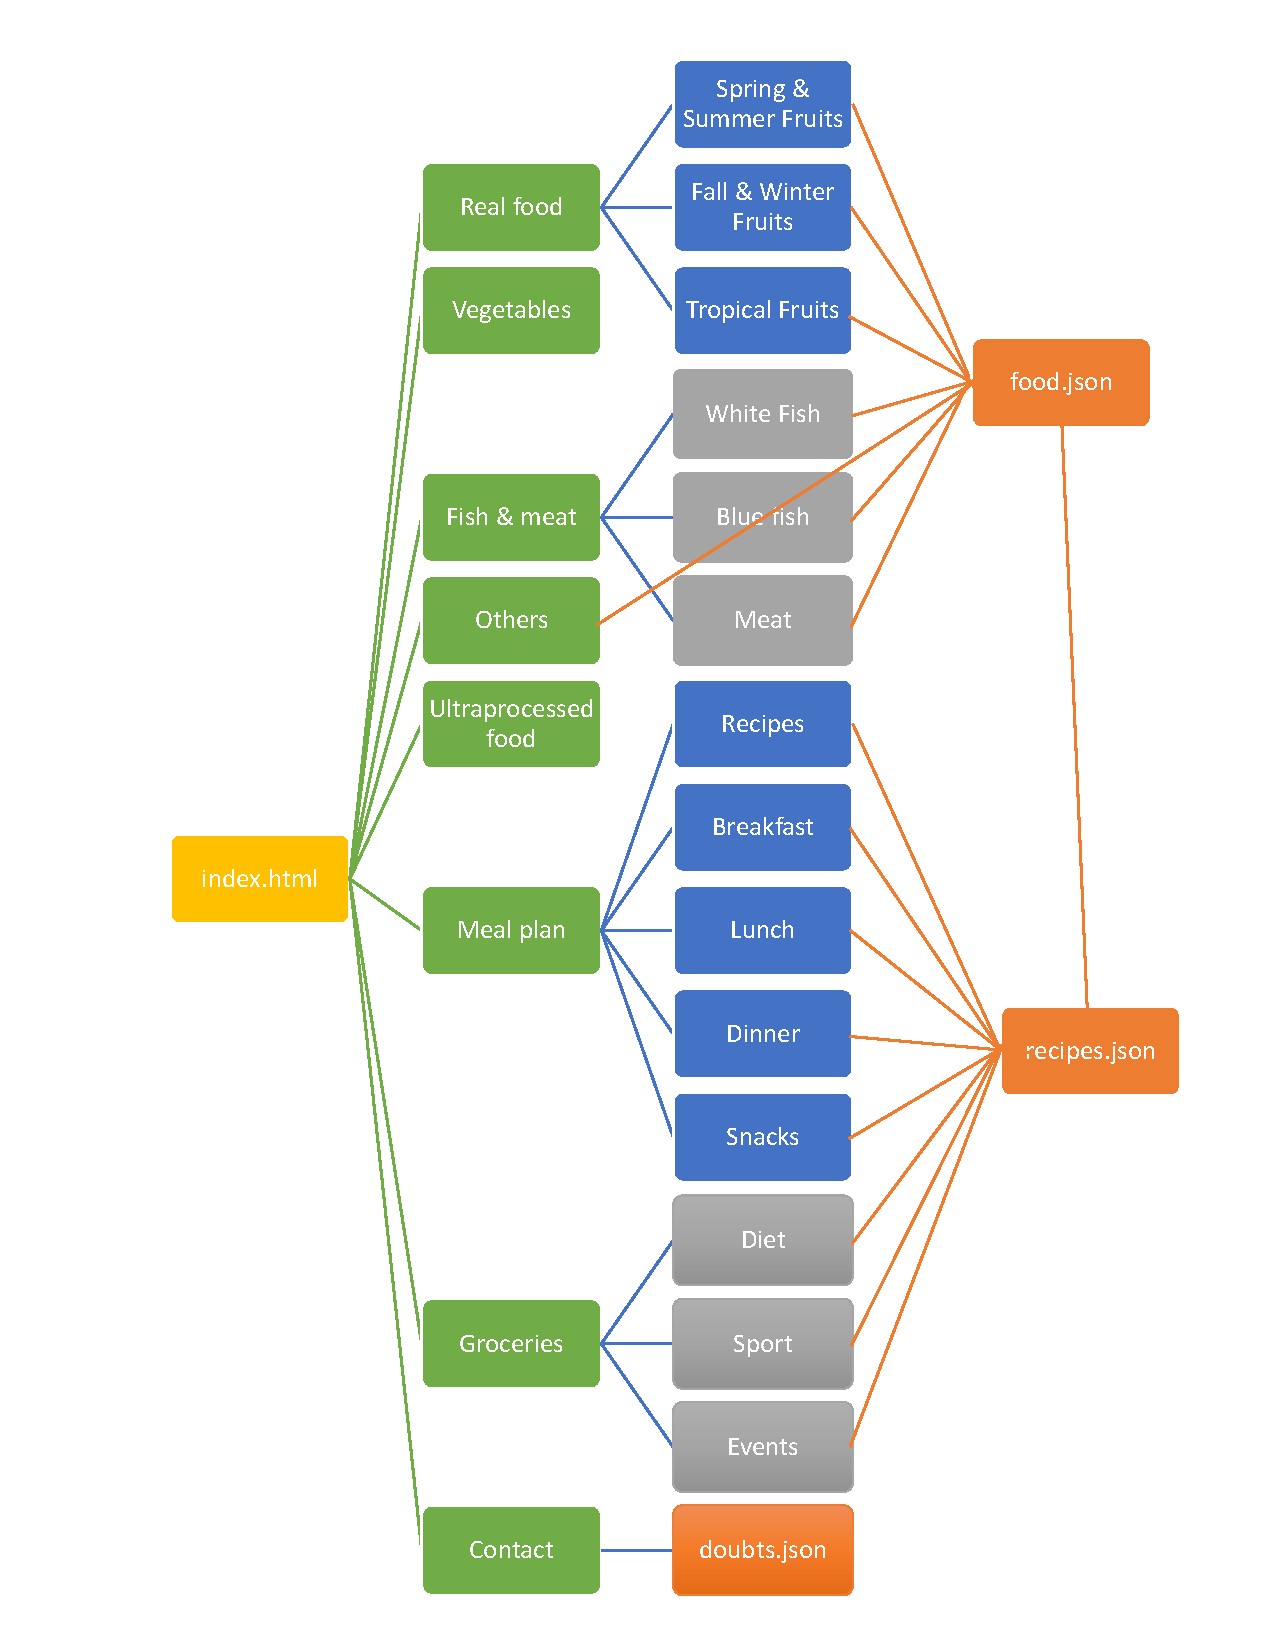
\includegraphics[width=8cm]{images/hierarchy.pdf}

    \textbf{Appendix 1 Navigation diagram}
    \vspace{2mm}

\end{document}
